\documentclass[addpoints,12pt,answers]{exam}
\usepackage{babel}
\usepackage[top=3cm,bottom=3cm,left=2.5cm,right=2.5cm]{geometry}
\usepackage[utf8]{inputenc}
\usepackage[T1]{fontenc}
\usepackage{booktabs}
\usepackage{graphicx}
\usepackage{csquotes}
\usepackage{paralist}
\usepackage{wasysym}
\usepackage[math]{iwona}
\usepackage{setspace}
\usepackage{enumitem}
\usepackage{multirow}

\pointpoints{Point}{Points}
\bonuspointpoints{Bonuspunkt}{Bonuspunkte}
\renewcommand{\solutiontitle}{\noindent\textbf{Solution:}\enspace}

\chqword{Frage}   
\chpgword{Seite} 
\chpword{Punkte}   
\chbpword{Bonus Points} 
\chsword{Erreicht}   
\chtword{Gesamt}

\checkboxchar{\Square}
\checkedchar{\CheckedBox}

\pagestyle{headandfoot}
%\runningheadrule
%\firstpageheader{ECO208}{Test 3}{28th Feb, 2022}
%\runningheader{ECO208}{Test 3}{28th Feb, 2022}
%\firstpagefooter{ECO208}{Test 3}{\thepage\,/\,\numpages}
%\runningfooter{ECO208}{Test 3}{\thepage\,/\,\numpages}
\doublespacing

\begin{document}
	\vspace*{3em}
	
	\makebox[\textwidth]{ECO 209  Practice Questions}
	\makebox[\textwidth]{Name:\enspace\hrulefill}
	
	\vspace*{3em}
	
	\begin{questions}
		

		\question Explain the difference between flow and stock measures of economic, while identifying specific examples. Include a discussion (again on the basis of specific examples) of how such a distinction might be critical for comparing patterns of macroeconomic well-being and growth for different countries, regions and/or individuals.
		\clearpage
		\textbf{Solution}
		Flow measures account for economic activity over a specified period, typically representing a rate of change or flow per unit of time. Examples of flow measures include: output, investment, etc
		
		Stock measures represent the accumulation of a particular economic variable at a specific point in time. Examples of stock measures include: Capital, debt, wealth
		
		When comparing the economic performance of countries or regions, flow measures like GDP growth rates provide insights into the economic activity over certain period. However, stock measures such as wealth/capital per capita offer a more comprehensive view of economic well-being, it shows the accumulated assets and resources available to individuals or nations.
		
		\clearpage
		\question  Determine the scale of return of the followings production function where Y is the output, N is the labour input and K is the capital input
		\begin{parts}
			\part $Y= A(N+K)^\alpha$
			\part $Y = (N^\alpha + K^\alpha)^{\frac{1}{\alpha}}$
			\part $Y = AN^{0.3} K^{0.7}$
		\end{parts}
		
		\clearpage
		\textbf{Solution}
		For each of the following we will multiple the input by $t$ times
		\begin{parts}
			\part $Y= A(N+K)^\alpha$
				\[Y= A(tN+tK)^\alpha = A t^\alpha (N+K)^\alpha\]
				It will depend on the $\alpha$.
				
				If $\alpha <1$, the function is decreasing return to scale
				
				If $\alpha =1$, the function is constant return to scale
				
				If $\alpha >1$, the function is increasing return to scale
			\part $Y = (N^\alpha + K^\alpha)^{\frac{1}{\alpha}}$
			\[Y = (N^\alpha + K^\alpha)^{\frac{1}{\alpha}} = \left((tN)^\alpha + (tK)^\alpha\right)^\frac{1}{\alpha} = \left((N^\alpha + K^\alpha) (t)^\alpha\right)^\frac{1}{\alpha} = t (N^\alpha + K^\alpha)^{\frac{1}{\alpha}}\]
				This function is constant return to scale
			\part $Y = AN^{0.3} K^{0.7}$
			
			\[Y = AN^{0.3} K^{0.7} = A(tN)^{0.3} (tK)^{0.7} = t AN^{0.3} K^{0.7}\]
			
			This function is constant return to scale
		\end{parts}
		
		\clearpage
		\question  List and explain three different ways that the government can finance their spending.
		
		\clearpage
		\textbf{Solution}
		\begin{parts}
			\part 	Increasing tax revenue: the government can finance its spending is by raising tax revenue. This involves imposing higher taxes on individuals, businesses, or certain economic activities to generate additional income for the government. 
			\part	Increase money supply: the government finance its spending is by increasing the money supply. This typically involves the central bank purchasing government securities. The government can then use this newly created money to finance its expenditures.
			\part	Increase the amount of government borrowing: increasing the amount of government borrowing. This entails the government issuing bonds or taking out loans from domestic or international sources to raise funds
		\end{parts}
		
		\clearpage
		\question  In a hypothetical economy, Eatonville, the output gap rise to 5\% during the Information Technology boom. Many people believe that the multiplier was equal to 3. Given the equations that describe the economy:
		
		\[C_t = \bar{a}_c \bar{Y}_t + \bar{x} \widetilde{Y}_t \bar{Y}\]
		\[I_t = \bar{a}_I \bar{Y}_t - \bar{b} \left(R_t - \bar{r}\right)\bar{Y}_t + 0.2\widetilde{Y} \bar{Y}_t\]
		\[G_t = \bar{a}_G \bar{Y}_t\]
		
		
		\begin{enumerate}[label=(\alph*)]
			\item \textbf{(2  pts)} What is value of $\bar{x}$? 
			
			\item \textbf{(1  pts)} What would the percent change in government expenditure be to close this gap, assuming monetary policy is not being used?
			
			\item \textbf{(2  pts)} Relying only on monetary policy and $\bar{b}=0.5$, what is the required real interest rate to close the gap? Assumes that initially, $R_t$ equals $\bar{r}$ (i.e., the boom is caused solely by a change in $\bar{a}$).
			
			\item \textbf{(1  pts)} Why does the government and central bank want to cool down the economic boom? How does the policy help achieve this target?
			
		\end{enumerate}
		
		\clearpage
		\textbf{Solution}
		\begin{enumerate}[label=(\alph*)]
			\item  \[3 = \frac{1}{1-\bar{x} - 0.2}\]
			\[\bar{x} = 0.466666666\]
			\vspace{1cm}
			\item  \[ \Delta a_G = -0.05/3 = -0.01667\]
			\item  We want to solve for $\Delta R_t$
			\[\widetilde{Y}_t = \frac{1}{1-\bar{x} - 0.2} \left[\bar{a}_t - \bar{b} \left(R_t-\bar{r}+\Delta R_t\right) \right] = 0\]
			\[\widetilde{Y}_t = 3 \left[-0.01667 - 0.5 \left(0-0.03333\right) \right] = 0\]
			
			\vspace{1cm}
			\item The government and central bank want to cool down the economy because they worry for the inflation. The policy would work because of the Phillip curve. When the economy is booming, the prices tend to increase as the firm need to hire more worker or increase costs to satisfy the demand.
		\end{enumerate}
%		\newpage 
%		\centering{This page intentionally left blank.}
%		\ % The empty page
		\clearpage
		\question Consider the consumption model discussed in Ch.16, the consumer has the following utility function:
		\[U = ln(c) + \beta ln(c')\]
		where $c$ is the consumption in the current period, $c'$ is the consumption in the future period and $\beta$ is the discount factor. The consumer has an initial assets of $f$ and can save or borrow $f'$ amount at interest rate of $r$. In current period, the consumer receive $y$ amount of income. In the future period, the consumer receives $y'$ amount of income. 
		
		The government decided to implement a form of wealth tax. It will charge $\tau f'$ in the current period. The $\tau$ is the percentage that the government is going to tax on the total saving in current period ($ f'$).
		
		\begin{enumerate}[label=(\alph*)]
			\item \textbf{(2 pts)} 	Setup the budget constraint. Shows the current period budget constraint, future period budget constraint and the lifetime budget constraint.
			
			\item \textbf{(4 pts)}  Derive the Euler equation and compute the optimal $c$ and $c'$ 
			

			
			\item \textbf{(4 pts)}  Now, the government decided to remove the wealth tax entirely (i.e., $\tau = 0$). Based on the equation derived, what is the effect on $c$ and $c'$. What is the intuition behind it? Explain in 3-5 sentences.
			
		\end{enumerate}
		
		\clearpage
		\textbf{Solution}
		\begin{enumerate}[label=(\alph*)]
			\item 			
			\[c= y+f-f' -\tau f'\]
			
			\[c'=y'+(1+r)f'\]
			
			\[c+\frac{c' (1+\tau)}{1+r} = y+\frac{y'(1+\tau)}{1+r} + f\]
			
			\item 
			The utility function:
			\[\ln\left(y + \frac{(1+\tau)y'}{1+r} +f - \frac{(1+\tau)c'}{1+r} \right) + \beta\ln(c')\]
			The first order condition w.r.t. c':
			\[\left(\frac{1}{c}\right) \frac{1+\tau}{1+r} = \frac{\beta}{c'}\]
			
			Rearrange:
			\[\frac{c'}{c} = \beta \frac{1+r}{1+\tau}\]
			
			Plug the Euler equation back to the budget constraint.
			
			\[c+\frac{ \beta \frac{1+r}{1+\tau} c (1+\tau)}{1+r} = y+\frac{y'(1+\tau)}{1+r} + f\]
			
			\[c+ \beta  c  = y+\frac{y'(1+\tau)}{1+r} + f \rightarrow c = \left(\frac{1}{1+\beta}\right) \left[y+\frac{y'(1+\tau)}{1+r} + f\right] \]
			
			, and
			\[c'= \beta \frac{1+r}{1+\tau}  \left(\frac{1}{1+\beta}\right) \left[y+\frac{y'(1+\tau)}{1+r} + f\right] \]
			

			\item
			If the $\tau=0$, consumer would consume more of future consumption. It is because of the positive substitution effect  and positive income effect. The consumer would have incentive to save more and consume more in the future. Meanwhile, the consume would reduce the current consumption, although consumer still has the positive income effect (less tax = higher income).
			
		\end{enumerate}
		
%		\clearpage
%		\question This question relates to the growth model discussed in Chapter 6. Terra Cotta, a closed economy without government spending, features a production function:
%		
%		\[Y_t = A_t K_t^{2/5} L_{y,t}^{3/5}\]
%		
%		Here, \(Y_t\) represents the output, \(K_t\) denotes the capital, \(L_{y,t}\) stands for the labor employed and $A_t$ stand for TFP (or stock of ideas) in period \(t\). Terra Cotta's capital accumulation follows the standard function:
%		
%		\[K_{t+1} = (1 - \delta) K_t + I_t\]
%		
%		In this equation, \(\delta\) represents the depreciation rate, and \(I_t\) represents the investment in period \(t\). The accumulation of ideas  following:
%		
%		\[\Delta A_{t+1} = \bar{z}A_t L_{a,t}\]
%		where $\bar{z}$ is the productivity of idea creation.
%		
%		The sum of numbers of workers ($L_{y,t}$) and researchers ($L_{a,y}$) equal to the total population: $L_{y,t} + L_{a,t} = \bar{L}$.  The labor supply is inelastic, with the economy consistently providing \(\bar{L}\) units of labor at any given wage. Meanwhile, there are $\ell$ proportion of the population work in the idea production. Terra Cotta's population save a proportion \(\bar{s}\) of their output for investment each period.
%		
%		\begin{enumerate}[label=(\alph*)]
%			\item \textbf{(2 pts)} Show and discuss why the growth rate of output ($g_Y$) and capital ($g_K$) are equal. 
%			
%
%			
%			%	\vspace{1cm}
%			
%			\newpage
%			\item \textbf{(2 pts)} If all inputs have double, how many time does output multiply? Is it constant return to scale?
%			
%
%			\item \textbf{(1 pts)} An important feature of the Romer growth model is the increasing return to scale. Does the mode presented in this question exhibit this feature? How?
%			
%
%
%			\item \textbf{(3 pts)} Show that the growth rate of ideas $g_A$ is determined by constants and express $g_Y$ as a function of $g_A$. Also, find the steady-state levels of \textit{output per worker}.
%		
%			
%			
%
%			\item \textbf{(3 pts)} 	The Terra Cotta government is going to implement a policy that encourage immigration to the country for a single period at period T. During this period, a proportion $\ell$ of immigrants will be engaged in idea production.
%			
%			Draw the transition in both output and output per person from the balanced growth path before the policy change to after the policy change. Label all axis and key points of interest. Provide a explanation in 3-4 sentences.
%			
%			
%
%			\item \textbf{(3 pts)} (Independent of part e)) Unfortunately, Terra Cotta experienced an earthquake that destroyed most of its capital stock at period T. On the bright side, none of the population was lost. 
%			
%			Draw the transition in both output and output per person from the balanced growth path before the  earthquake to after the earthquake. Label all axis and key points of interest. Provide a explanation in 3-4 sentences.
%			
%		\end{enumerate}
%		
%		\textbf{Solution}
%		\begin{enumerate}[label=(\alph*)]
%			\item 
%			
%			Convert the production function into growth rate
%			\[
%			g_{Yt} = g_{At} + \frac{1}{4} g_{Kt} + \frac{3}{4}g_{L_{yt}}
%			\]
%			
%			The change in the capital stock is determined by investment minus depreciation:
%			
%			\[
%			g_{Kt} = \frac{\Delta K_{t+1}}{K_t} = \bar{s} \frac{Y_t}{K_t} - \delta
%			\]
%			
%			For \(g_{Kt}\) to be constant, the right-hand side must also be constant. Given that \(\bar{s}\) and \(\delta\) are constants, \(\frac{Y_t}{K_t}\) must be constant. This condition is met only if \(Y_t\) and \(K_t\) are growing at the same rate. If \(Y_t\) were growing at a faster rate, the ratio \(\frac{Y_t}{K_t}\) would increase each period. Therefore, it follows that \(g_K^* = g_Y^*\).
%			
%			
%			%	\vspace{1cm}
%			
%			\newpage
%			\item 
%			
%			\[A_t (2 K_t)^{2/5} (2L_{y,t})^{3/5} = 2 A_t (K_t)^{2/5} (L_{y,t})^{3/5} = 2Y_t\]
%			
%			It is constant return to scale.
%			
%			\item \textbf{(1 pts)} An important feature of the Romer growth model is the increasing return to scale. Does the mode presented in this question exhibit this feature? How?
%			
%			\textbf{Soln}
%			
%			Yes. It is because the $A$ is also growing.
%			
%			\clearpage
%			\vspace{6cm}
%			\item 
%			Researchers are used to produce new ideas:
%			\[g_{At} = \frac{\Delta A_{t+1}}{A_t} =\bar{z} L_{at} = \bar{z} \bar{\ell} \bar{L} = \bar{g}\]
%			
%			Now, we know that $g_{At}$ is a constant.
%			
%			Plug in $g_{At}=\bar{g}$, $g_K^* = g_Y^*$ and $g_{Lyt} = 0$,
%			\[g_{Y}^* = \bar{g} + \frac{1}{4} g_{Y}^* + \frac{3}{4}0 \rightarrow g_{Y}^* = \frac{4}{3}\bar{g} = \frac{4}{3}\bar{z} \bar{\ell} \bar{L}\]
%			For the long-run combined model, this equation pins down	the growth rate of output and 	the growth rate of output per person
%			
%			
%			Now, we know that $g_Y^*$ is a constant along a balanced growth path. This implies
%			\[\frac{K^*_t}{Y^*_t} = \frac{\bar{s}}{g_Y^* + \delta}\]
%			This solution can be substituted back into the production function and solved to get
%			\[y^*_t = \frac{Y_t^*}{\bar{L}} = \left(\frac{\bar{s}}{g_y^* +\delta }\right)^{1/3} A^{*4/3}_t (1-\bar{\ell})\]
%			
%			
%			\newpage
%			\item 
%			
%			Since there are the same right proportional increase in the worker in the production sector. The output would increase proportionally to the increase in population. As a result, there are no change immediately for the output per capita. However, as the popualtion increase, there would be an increase in the total output. 
%			
%			After the initial period, the growth rate would be higher as more people are in the research sector. More idea can be shared. Therefore, the both output and output per capita would grow faster after the initial period.
%			
%			\begin{figure}[htbp!]
%				\centering
%				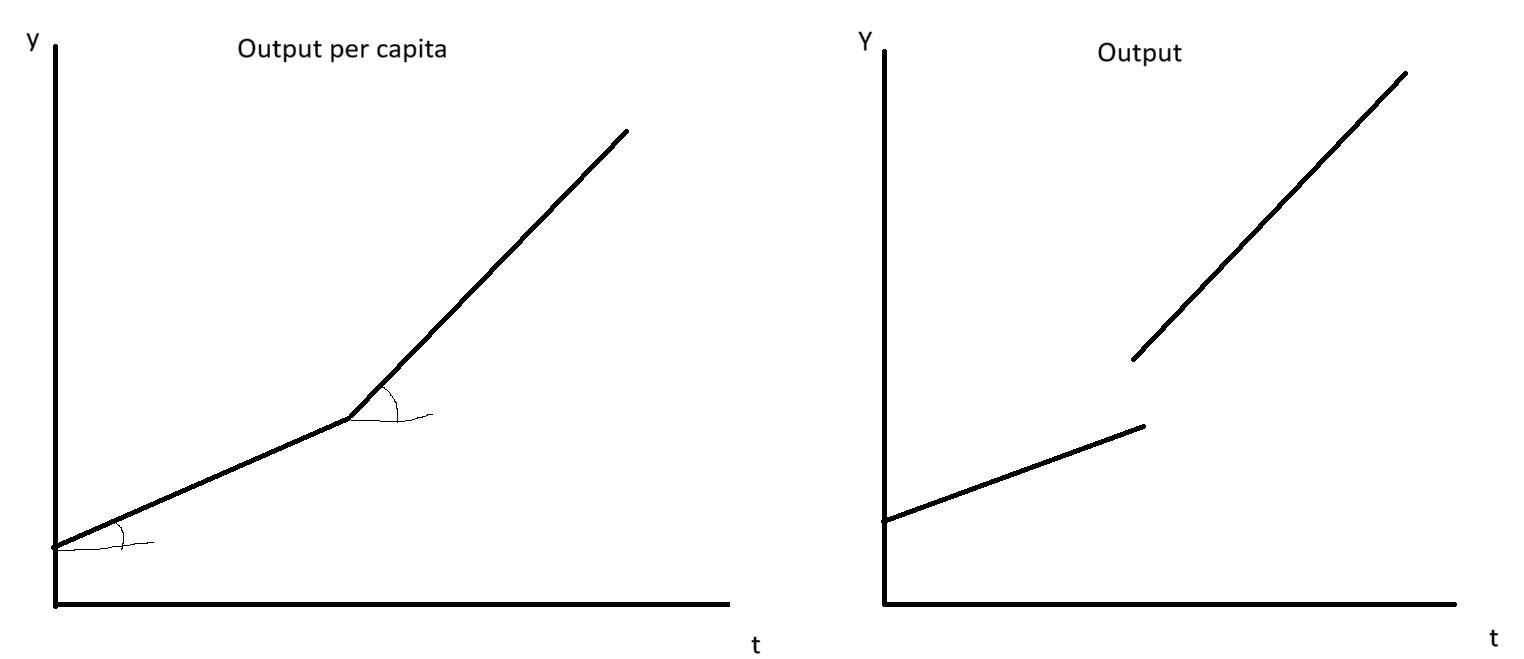
\includegraphics[width=0.8\linewidth]{figure/a6e}
%			\end{figure}
%			
%			
%			
%			\newpage
%			\item 		
%			When the capital got destroyed, the output would be lower right away in both output and output per capita. The economy will invest more into capital as the MPK rise.  Therefore, the growth would be faster until it reaches its balance growth path.
%			
%			\begin{figure}[htbp!]
%				\centering
%				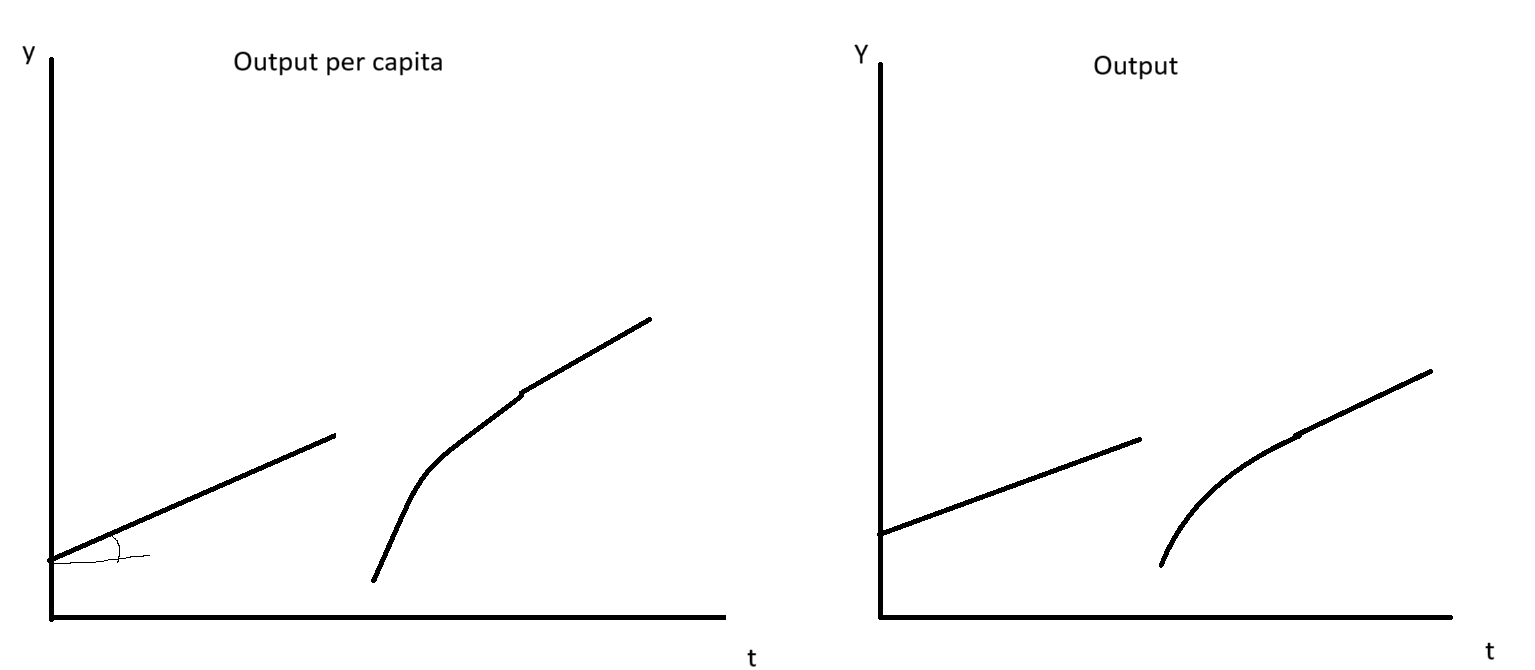
\includegraphics[width=0.8\linewidth]{figure/a6f}
%			\end{figure}
%			
%			
%		\end{enumerate}
%		
		\clearpage
		\vfill
		
		 \centering{-- The End -- }
		
		
		
		%		\begin{solution}
			%			
			%		\end{solution}	
%		\clearpage 
%		
%		\question Was wäre, wenn es keine Luft gäbe?
%		\begin{parts} 
%			\part[5] Was würde mit Luftballons geschehen? 
%			\bonuspart[6] Wie könnten Fluggesellschaften damit umgehen?
%		\end{parts}
%		
%		\question [100] Wird es morgen schneien?
%		\begin{checkboxes}
%			\CorrectChoice Ja
%			\choice Nein
%			\choice Vielleicht
%		\end{checkboxes}
%		
%		\question Ein Name der folgenden Reihe passt nicht zu den anderen. Welcher?
%		\begin{oneparchoices}
%			\choice Donald
%			\choice Dagobert
%			\choice Daisy
%			\choice Micky
%			\CorrectChoice Balu
%		\end{oneparchoices}
		
	\end{questions}
	
%	\begin{center}
%		\combinedgradetable[h][questions]
%	\end{center}
	
\end{document}